
%\newpage
\section{Measurement of frequency}
\label{sec:frequency}

Beginning with Version 1.10k the frequency measurement can be selected with a control menu.
The normal frequency measurement is done with counting the falling edges of input signal T0 (PD4)
with counter 0 for one second. For maintaining of a accurate second, the counter 1 is used
with a 256:1 prescaler of the CPU frequency. 
The 16 bit counter of the ATmega can be used up to \(16MHz\) CPU frequency with the prescaler to
serve the second period in one pass.
For the start and stop of the counter 0 ist the compare register B and A of the counter 1 used.
To prevent a unstable delay by polling the compare event signals, for starting and stopping the
Interrupt Service of both counter 1 compare events is used.
The time delay of both Interrupt Service Routines is nearly equal.
To maintain a accurate second period is a constant delay insignificant.
With analysing the assembler code, the difference in time can be adjusted.\\

For frequencies below \(25kHz\) the normal measurement is followed by a measurement of
period time. This additional measurement is only followed after a normal frequency measurement.
This will be done by measuring the time of a selectable count of the Pin Change interrupts
of the PCINT20 (PD4) input with the counter 0.
By measuring the period both, the negative puls width and the positive puls width, should be
at least \(10\mu s\) .
The counter 0 is used with full clock rate. This results to a resolution of \(125ns\) for
\(8MHz\). With a greater count of measurements periods the resolution can be reduced.
By using a measurement period of 125 periods, the middle resolution for one period is \(1ns\).
To prevent the inexactness of start and stop the counter 0, the start of counter 0 is started
within the first pin change interrupt of PCINT20 and will be stopped with the last pin change interrupt
with the same interrupt service routine.
The count of periodes is choosed, that the measurement time is about 10 million clock tics.
The part of error from one clock is only 0.1ppm with this choise.
With a \(8MHz\) clock the measurement time is about 1.25 seconds.
From this mean value of one period a frequency with better resolution is computed too.

For checking the procedure, two testers are measured against each other.
First the test frequencies are generated with tester 2 and measured with tester 1.
After that the testers are swapped and the measurement is repeated.
Figure \ref{fig:freq-ppm} shows the results of both measurement series.
The nearly constant errors can be explained with a little frequency difference of both crystals.

\begin{figure}[H]
\centering
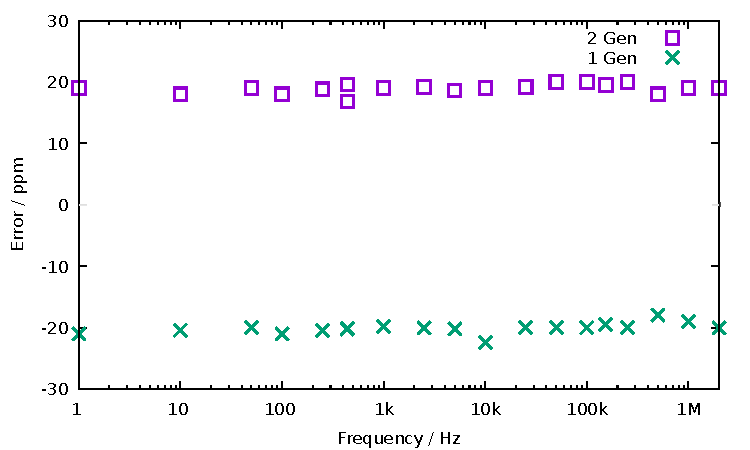
\includegraphics[width=1.\textwidth]{../GNU/frequency-ppm.pdf}
\caption{Relativ erros of frequency measurement}
\label{fig:freq-ppm}
\end{figure}

\subsection{Calibration of frequency with a GPS- or GLONASS-receiver}

Tuning of the cystal frequency is possible with a adjustable capacitor (5-25pF) at the crystal.
The one pulse per second (1PPS) from the GPS receiver \textbf {UP501} from \textbf {Fastrax Ltd.} and from the GPS/GLONASS receiver
\textbf {GNS701} from \textbf {Global Navigation Systems GmbH} has been tested successfully for the calibration of the
crystal frequency.
The measured period could be adjusted to exactly \(1000.000ms\).
Only the last digit can toggle with one unit.
Of course the frequency of the crystal is temperature dependent.
Therefore you can not expect a very good long time stability.

The figure \ref{fig:GPS-1PPS} shows the used circuits with a UM232 USB-serial converter
as connection of the receiver modules to a computer.
The UM232 converter support the circuit sowohl with both, the \(5V\) and the \(3.3V\) supply voltage
from the USB supply voltage.
No connection to a computer is required for operating the receivers.
Only the \(5V\) supply voltage must be provided to the USB connector.

\begin{figure}[H]
  \begin{subfigure}[b]{.5\textwidth}
    \centering
    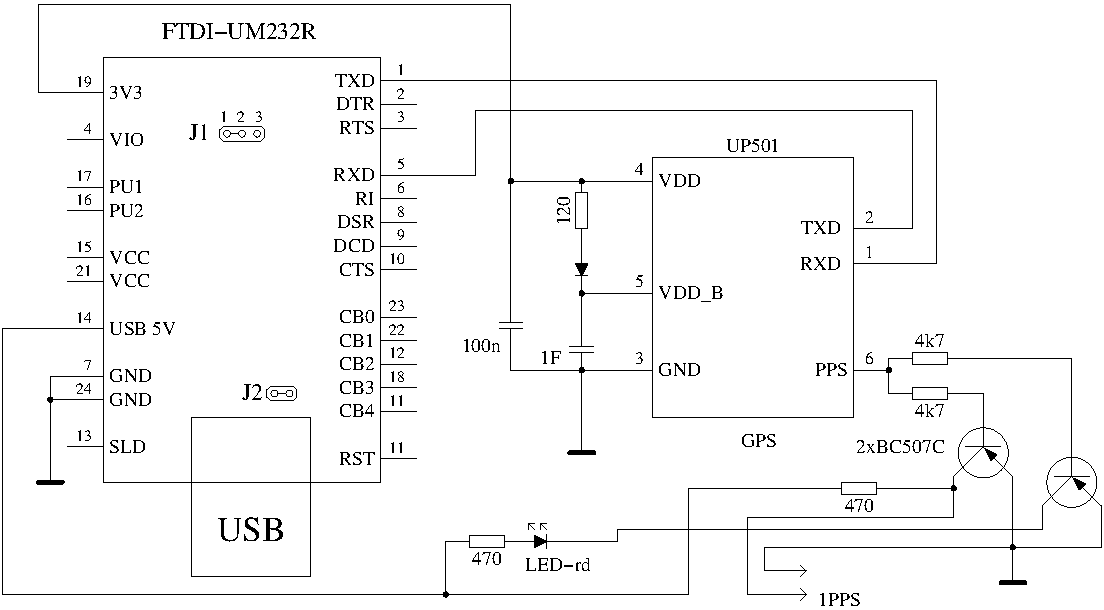
\includegraphics[width=.95\textwidth]{../FIG/GPS_UP501.pdf}
    \caption{GPS}
  \end{subfigure}
  ~
  \begin{subfigure}[b]{.5\textwidth}
    \centering
    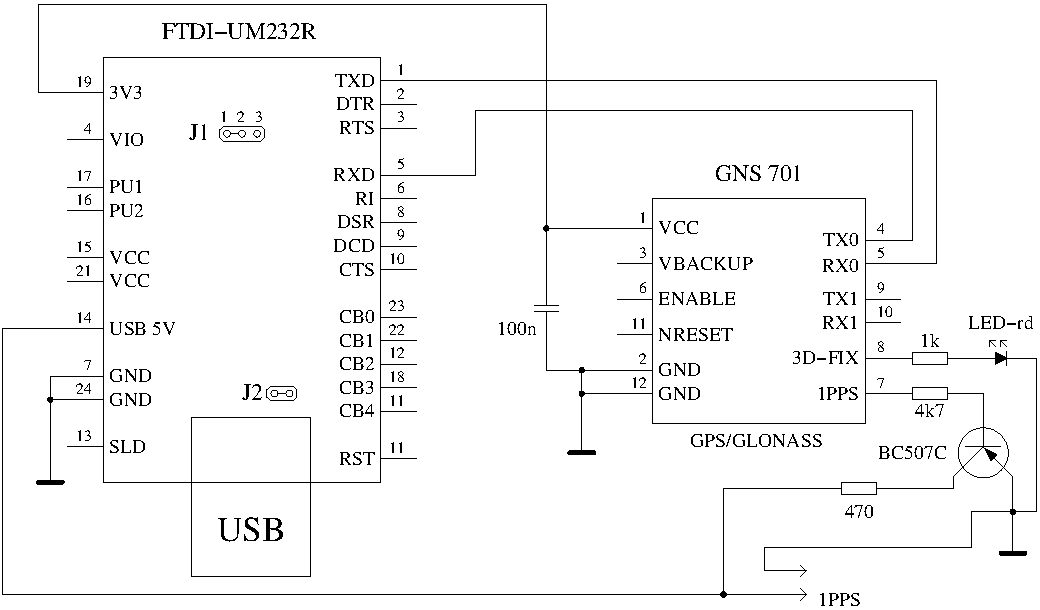
\includegraphics[width=.95\textwidth]{../FIG/GPS_GNS701.pdf}
    \caption{GPS/GLONASS}
  \end{subfigure}
  \caption{Generation of a 1PPS signal with GPS receiver }
  \label{fig:GPS-1PPS}
\end{figure}

\subsection{Calibration of the crystal frequency with a clock modul}

To tune the crystal frequency of the transistor tester you must first exchange one of the
crystal capacitors against a trimmer with adjustable capacity.
The advantage of using watch modules for frequency calibration instead of GPS or GLONASS modules is,
that you need no clear view to sky. You can adjust the frequency nearly at any place.
I examined watch modules with a DS3231 chip and a printed board labled with ''ZS-042''.
The examined moduls are probably build in china and are all of the boards are equipped
with a DS3231M chip. The DS3231M chip use a MEMS (Micro Electro Mechanical System) resonator 
instead of the DS3231SN chip, which use a crystal with \(32768Hz\).
A simular MEMS resonator is also used by the DCP1301 chip.
The picture~\ref{fig:DS3231M} shows one of the used modules.

\begin{figure}[H]
\centering
\includegraphics[width=.6\textwidth]{../PNG/DS3231M.jpg}
\caption{One example of the examined DS3231 modules}
\label{fig:DS3231M}
\end{figure}

Both DS3231 chip versions use a internal temperature measurement to control the frequency of
the time base in a manner, that the frequency drift with temperature is nearly
perfect compensated in a wide range.
Unfortunately the provided \(32kHz\) Signal of the DS3231M chip can not be used for a
frequency calibration. I have measured different frequencies of \(32641Hz\), \(32710Hz\),
\(32730Hz\) and \(32748Hz\) for all four tested modules. 
All of these Frequencies are far away from the expected exactly \(32768Hz\).
If you connect the modules to a Arduino UNO, you can also enable a 1PPS (\(1Hz\)) output
to the SQW pin.
This output is so stable and exactly, that it can be used for the calibration.
The data sheet of the DS3231M promise for the 1PPS output a accuracy of \(pm 5ppm\) for
the full temperature range of \(-45\celsius\) to \(+85\celsius\), while the accuracy of the
\(32kHz\) output is only specified to \(\pm 2.5\%\) (\(25000ppm\)).

The data sheet of the DS3231SN chip promise a accuracy of \(pm 3.5ppm\) for the full
temperature range from \(-40\celsius\) to \(+85\celsius\) and a accuracy of \(\pm 2ppm\)
for the temperature between \(0\celsius\) to \(+40\celsius\).
The DS3231SN chip use a internal clock crystal with a frequency of \(32768Hz\), which is
controlled with switchable capacitors over a wide temperature range.
With the known temperature drift of the crystal and a build in temperature measurement
the frequency of the controlled crystal is nearly constant.
To examine these chips too, I have replaced the DS3231M chips by DS3231SN chips for
all four modules.
With a fresh calibrated transistor tester (\(16MHz\) model) I have measured the output frequency of all
modules with the same result of \(32.76800kHz\). Very rarely a differerence of \(0.03Hz\)
was shown during the measurements. This is only a difference of \(1ppm\).
A fractional amount of \(1Hz\) is only shown, if the frequency is calculated of a period measurement.
The limit for period measurement is changed from \(25kHz\) to \(33kHz\) to enable
the period measurement for the \(32768Hz\) signal.

